%%%%%%%%%%%%%%%%%%%%%%% file template.tex %%%%%%%%%%%%%%%%%%%%%%%%%
%
% This is a general template file for the LaTeX package SVJour3
% for Springer journals.          Springer Heidelberg 2010/09/16
%
% Copy it to a new file with a new name and use it as the basis
% for your article. Delete % signs as needed.
%
% This template includes a few options for different layouts and
% content for various journals. Please consult a previous issue of
% your journal as needed.
%
%%%%%%%%%%%%%%%%%%%%%%%%%%%%%%%%%%%%%%%%%%%%%%%%%%%%%%%%%%%%%%%%%%%
%
% First comes an example EPS file -- just ignore it and
% proceed on the \documentclass line
% your LaTeX will extract the file if required
\begin{filecontents*}{example.eps}
%!PS-Adobe-3.0 EPSF-3.0
%%BoundingBox: 19 19 221 221
%%CreationDate: Mon Sep 29 1997
%%Creator: programmed by hand (JK)
%%EndComments
gsave
newpath
  20 20 moveto
  20 220 lineto
  220 220 lineto
  220 20 lineto
closepath
2 setlinewidth
gsave
  .4 setgray fill
grestore
stroke
grestore
\end{filecontents*}
%
\RequirePackage{fix-cm}
%
\documentclass{svjour3}                     % onecolumn (standard format)
%\documentclass[smallcondensed]{svjour3}     % onecolumn (ditto)
%\documentclass[smallextended]{svjour3}       % onecolumn (second format)
%\documentclass[twocolumn]{svjour3}          % twocolumn
%
\smartqed  % flush right qed marks, e.g. at end of proof
%
\usepackage{mhsetup}
\usepackage{amsmath}
\usepackage{mathtools}
\usepackage{natbib}
\usepackage{graphicx}
\usepackage{float}
\usepackage{qtree}
\usepackage[utf8]{inputenc}
\usepackage{gb4e}
\usepackage[T1]{fontenc}
\bibpunct{(}{)}{,}{a}{}{,}
\newcommand{\noteme}[1]{\noindent \textbf{[[JCW:  #1 ]]}}
\renewcommand{\theequation}{\Alph{equation}}

% Insert the name of "your journal" with
\journalname{Journal of }

\begin{document}

\title{Optionality is Stable Variation is Competing Grammars
\thanks{...All errors are the second author's.}}
%\subtitle{Do you have a subtitle?\\ If so, write it here}

%\titlerunning{Short form of title}        % if too long for running head

\author{Josef Fruewald \& Joel C. Wallenberg}

%\authorrunning{Short form of author list} % if too long for running head

\institute{Joel C. Wallenberg \at
              Newcastle University \\
              Tel.: +44-(0)191-222-7366\\
              \email{joel.wallenberg@gmail.com}
}

\date{Received: date / Accepted: date}
% The correct dates will be entered by the editor


\maketitle

\begin{abstract}
stuff
\keywords{syntax \and morphology \and language change \and language acquisition \and evolutionary dynamics}
% \PACS{PACS code1 \and PACS code2 \and more}
% \subclass{MSC code1 \and MSC code2 \and more}
\end{abstract}

\section{Introduction}
\label{intro}

This is a strictly Minimalist proposal, in the sense of \citet{chomsky1993, chomsky1995, chomsky1998,chomsky2001}.
It takes an issue which has frequently been brute-force encoded in the grammar with little explanatory content, namely optionality, and shows how it can be fully explained as an effect of the interface between the narrow grammar and general properties of the linguistic, cognitive, and social systems in which the derivation is produced.
Our proposal is also not to postulate a set of \textsl{ad hoc} interface constraints; the phenomenon which appears to be optionality in the phonology and syntax is an interface \textsl{effect}, a by-product of how the derivation must relate to independently motivated linguistic and extralinguistic structures.

In this study, we consider four case studies, two syntactic and two morphophonological, which have been described either as diachronically stable variation or as optional operations: \textsl{-in}/\textsl{-ing} variation, Heavy NP Shift (or DP extraposition), [t]/[d]-deletion, and English topicalization (object DP fronting).
Each case involves a probabilistic (i.e. ``optional'') alternation between surface variants, and we show that they are all best understood as instances of an independently attested phenomenon, the alternation between linguistic variants which is observed during a language change in progress.
This is the change-related alternation which is usually called ``competing grammars'' \citep[][]{kroch1989}, which can be defined as the occurrence of alternative atomic units/rules of grammar in a single speaker's inventory, and is usually diachronically unstable.
In fact, the Minimalist research program demands that such a reduction be attempted, and the state of the art in the current  theory of functional heads and movement already predicts that syntactic optionality is the same as competing grammars (i.e. morphosyntactic doublets), though few researchers to date have noticed this \citep[with the exception of][]{kroch1994}.
We also show that even though grammatical optionality is really the same phenomenon as a language change in progress, the competing grammars situation can become diachronically stable under a very specific (and perhaps rare) set of circumstances: when the two variants have partially specialized along a continuous dimension of use with no clear endpoints (e.g. style, phonological heaviness).
  
In the first section below, we introduce the problem of stable variation in the sociolinguistic and phonological literature, and show how it relates to syntactic optionality.
In particular, we show how optionality in syntax can only be described in a Minimalist framework as doublets of functional heads, which is really the same as competing grammars, and that this poses a problem for language acquisition.
In section (\ref{solution}), we show that stable variation can persist just in case the variants become specialized in use along a particular type of continuous dimension.
Section (\ref{cases}) presents our case studies, and shows how they are all situations in which variants have become semi-specialized along a continuous dimension of use, which is the only circumstance that could allow such variation to persist indefinitely.
Lastly, we conclude and offer some predictions that this approach makes for future research.


\section{The Problem of Stable Variation}
\subsection{Optionality in Minimalism}

An important unification of different aspects of language change was presented in \citet{kroch1994}.
\citet{kroch1994} showed that syntactic variation and change can be viewed as the same phenomenon as morphological variation and change, i.e. morphological doublets where morphological features are spelled out in two alternative ways, such as \textsl{dive}/\textsl{dove}.
Kroch presents his view of the ``Blocking Effect'' (see references in \citealt{kroch1994} for the history of this idea), which he explains as a diachronic pressure for morphological doublets to disappear over time.
Though any individual can learn synonyms or alternate spell-outs for the same morphological features, the alternatives do not stably coexist over long periods of time.
Rather, one alternative replaces the other, or the two alternatives specialize in some way so that they no longer overlap in use.
This specialization can be the reanalysis of one variant as spelling out a different set of morphological features, but it does not need to be reanalyzed in that very specific sense: as long as the variants become restricted to non-overlapping contexts, they no longer ``block'' each other, i.e. compete for use.

The key insight of \citet{kroch1994} is that in a Minimalist syntactic system, the Blocking Effect of diachronic morphology (or synonyms generally) applies straightforwardly to the syntax as well.
In Minimalism, the syntax is a very generalized process of combining and projecting syntactic heads.
Thus, syntactic parameters (e.g. word order) must be the exponents of features on the syntactic heads, which then show themselves as these heads combine with complements and project, etc.
In this way, variation between two word orders such as OV and VO is really the same as a morphological doublet: the ``competing grammars'' \citep{kroch1989} are just alternative featural versions of a single syntactic head, e.g. $v$, and whichever version is used in a given sentence leads to certain effects on the rest of the structure and the resulting string.
The diachronic instability of having multiple versions of the same basic head is then just the Blocking Effect from morphology, and needs no additional statement in a theory of language change: there is a pressure against different exponents for the same meaning and function, because they ``block'' each other and compete for use.
Just as in morphology, one syntactic variant will replace the other, unless the two versions of the relevant head somehow specialize such that they no longer overlap in use (and Kroch gives some examples where this seems to have occurred in the syntactic domain).

In a Minimalist syntax, the trigger for any movement can only be the featural content of some functional head \citep{chomsky2000, chomsky2001}.
Combined with Kroch's (1994) analysis of syntactic change, this idea has a consequence that Kroch did not consider: all ``optional'' syntactic operations must also be instances of competing grammars (i.e. morphosyntactic doublets), and vice-versa.
A maximally simple syntactic system has a great deal of predictive power because of its inherent rigidity, and such a theory accordingly does not leave many possible analyses of an optional movement phenomenon.
A Minimalist syntax does not allow for any construction-specific transformational rules, only one generalized transformation for putting syntactic pieces together: Merge (with Move actually being subtype of Merge, either combined with Agree, as in \citealt{chomsky2000}, or not, as in \citealt{chomsky2004, chomsky2008}).
When a head, H, has projected once (H'), it can combine with a specifier and project again either by Merge (external) or Move.
What determines whether Merge or Move is used, or indeed, whether the head projects again at all, is whether the head has a feature which must be checked against a particular type of XP in a spec-head configuration.
So far so good, for obligatory movements.
If H has a certain feature, F, then the movement occurs; otherwise, the movement does not.
Because the default in a maximally simple (i.e. Minimalist) system is no movement at all, there is simply no way to encode optional movement with a feature.
(Note that ``Merge...preempts Move'' requires no movement to be a default in the system, as initially pointed out in \citealt{chomsky2000}.)

The only way to state an optional movement in such a syntactic system, without adding new theoretical machinery, is by allowing the speaker's inventory of functional heads to include two flavors of the same functional head H, one with the movement-triggering feature F and one without F.
The speaker can then choose to form a numeration with one version of H or the other.
This is a morphosyntactic doublet, by definition, of the same type discussed in Kroch (1994): 2 formal variants with no difference in meaning and overlapping discourse environments.
One could certainly imagine adding new mechanics to the syntax to encode optionality directly, and the literature is full of proposals such as: getting around the idea that no movement is a default, adding some kind of stochasticity to the features on heads themselves, or adding a whole post-processing system consisting of probabilistic trans-derivational filters \noteme{maybe cite someone for these}.
However, the simple Minimalist system is interesting precisely because it restricts our analytical possibilities and makes certain predictions as a result, so perhaps we should pursue this particular consequence of the system before complicating it.

Consider the English ``topicalization'' construction, as shown in the final sentences of (\ref{princetop1}) and \ref{princetop2}) below.

\begin{exe}
\ex \label{princetop1} She's going to use three groups of mice.
One, she'll feed them mouse chow, just the regular stuff they make for
mice.
Another she'll feed them veggies.
And the third she'll feed junk food.\\

\ex \label{princetop2} She was here two years.
[checking transcript] Five semesters she was here.\\
\citep[][8,9]{prince1999} 

\end{exe}

\noindent As was well-known even in the early days of generative syntax, English allows objects (and other XPs) to be fronted to a specifier position in the high left-periphery in certain discourse contexts.
For simplicity's sake, I will describe the construction as fronting to Spec, C (the standard assumption prior to \citealt{rizzi1997}), though the exact position targeted by the movement is not relevant to the question at hand.
\citet{prince1985,prince1998, prince1999} shows that this fronting is felicitous in two English discourse contexts, both of which require a certain type of contrast to appear on the fronted XP, though one context involves a backgrounded (i.e. topical, assumed) XP and the other an XP with information-structural focus (a distinct notion to contrast); these two contexts are shown in (\ref{princetop1}) and \ref{princetop2}), respectively.

However, even in these two contexts where topicalization is felicitous, it is never obligatory.
Leaving the XP \textsl{in situ} is equally felicitous, provided that the same accent pattern is maintained.
Thus, as long as the XP in question is accented, and as long as \textsl{junk food} is also in (\ref{princetop1}), the same sentences minus the fronting can be used in the same discourse context, as shown below.\footnote{Perhaps the required prosody is somewhat more awkward with this word order, leaving the object \textsl{in situ}.
Similarly, the \textsl{in situ} versions of (\ref{dem1}) and (\ref{dem2}) definitely require a different prosody from the fronted versions shown below.
These are both important points, and we return to the prosodic issue in section \ref{topsect} below.} To these two versions of this construction, \citet{caitldiss} adds a third context which involves a demonstrative being fronted, as shown in the two sentences below.


\begin{exe}
\ex \label{dem1} I promised that, if you voted in favour, I would respectfully ask UCU's forthcoming Congress to agree the changes.
This I will now do.\\
(UCU General Secretary, Sally Hunt)
\ex \label{dem2} I would do the following experiment.
This, only some people seem to be able to see,... and others not.\\
(Richard Feynman, Lecture on Color Vision, Caltech, March 6, 1962)
\end{exe}

\noindent \citet{caitldiss} argues extensively that even though these examples do not show the same type of contrast (or the same accent) on the fronted object as (\ref{princetop1}) and (\ref{princetop2}), the demonstrative itself is inherently contrastive, and this licenses the fronting construction.
Again, the sentences would be perfectly felicitous in context if the demonstrative were not fronted, and the meaning is apparently unchanged.
Thus, the fronting is truly optional.

Keeping the syntactic system as simple as possible, the movement to Spec, C must be triggered by some feature on C which attracts an XP to value its feature.
For simplicity's sake, I will follow \citet{caitldiss} and assume that some notion of contrast (though a subtle one) defines the set of XPs which could be fronted in the English topicalization construction, and these XPs bear a feature like [constrast].
When the fronting occurs, it is because there is a version of C in the phrase structure which probes for an XP bearing the feature [contrast].
In that case, it must attract the XP to its specifier.
In the situation where the fronting does not occur, this is only possible if a different version of C is used which is not a Probe for [contrast].
Thus, there are two versions of C in the speaker's inventory of functional heads, and the construction is the result of the speaker choosing a particular version to include in the numeration.
This is by definition a morphosyntactic doublet: two heads which differ only in formal syntactic features, and which overlap in use (both in their position in the structure and in this particular information-structural context).\footnote{Note that my basic argument is unaffected if one assumes that topicalization is the result of an ``edge feature'' (EF) on C, as suggested in \citet[][151]{chomsky2008}.
There would still have to be two versions of C, one with the EF, and one without the EF (or equivalent).
Though \citet{chomsky2008} does not deal with this explicitly, if topicalization were due to an EF, there would still need to be some mechanism for specifying the version of C that is used when no type of fronting to Spec, C takes place at all.} 

If syntactic change involves functional-head variants competing for use (i.e. competing grammars, doublets), in fact a kind of partial bidialectalism (in part of the system), and optional syntactic processes can only be described as functional-head variants competing for use, then all optional syntactic processes are actually a form of partial bidialectalism.
Why do we find this idea so difficult to swallow? Probably only because it offends our naive intuitions about our own linguistic competence.
But since intuiting how the brain works is notoriously unreliable for any brain-process that has been studied, and our idea is certainly no more counterintuitive than the rather baroque organization of the mammalian visual system (both in the eye and in the brain), we suggest that it is worthwhile to suspend disbelief and see if the competing grammars analysis of optionality makes any interesting predictions.
Theoretically, it is certainly a nice result, since we no longer need different machinery to account for change over time and synchronic optionality.


One prediction is immediately clear and, we hope, testable: \citet{kroch1989,kroch1994} states that the morphosyntactic doublet situation is inherent unstable over time.
Either the members of the doublet specialize in use, or the doublet resolves with one member taking over the entire function and causing the other member to drop out of use entirely.
It follows that optional syntactic processes are also inherently unstable over time, and one of these two outcomes should hold for the two syntactic options.
How then can anything like an optional syntactic movement exist for a long period of time (or an optional phonological rule, for that matter)? This is the question which the rest of the article addresses.
We suggest that it cannot exist stably over time, unless it undergoes some process of specialization for a particular environment or function.
If a process (or construction) remains stochastic (i.e. optional) in its behavior over time without fully specializing, the only way this situation can be maintained is if the process is \textbf{partially} specialized, but along some dimension of use which will not allow the construction to fully specialize because of some characteristic of the dimension itself.

\subsubsection{Expanding the Argument to Phonology}
It is worth noting that two of our case studies are morphophonological processes: {\sl -in}/{\sl -ing} Variation and {\sl t}/{\sl d} Deletion.
Approaches to explaining variation within phonology, either stably optional or changing, have largely differed from approaches within syntax.
The tendency has largely been to incorporate probabilities into the grammatical statements of the variable processes.

Take, for example, the finely articulated specification of a variable rule from \citet{3288} for {\sl t}/{\sl d} Deletion in African American English.
\begin{exe}
 \ex $\left[\begin{array}{rl}
	-&\mbox{cont}\\
	-&\mbox{grav}\\
	-&\mbox{nas}\\
	-&\mbox{comp}
\end{array}\right] \rightarrow (\emptyset) / 
\left[
	\begin{array}{rl}
		\alpha & \mbox{cons}\\
		\zeta &  \mbox{obstr}
	\end{array}
\right]\gamma(\mbox{+})\delta(\mbox{+})
\left[
	\begin{array}{l}
	\underline{\hskip 35pt}\\
	\epsilon~\mbox{voice}
	\end{array}
\right]
\beta(\sim \mbox{V})$ \label{variable.rule}
\end{exe}
The variables, $\alpha, \beta, \gamma \ldots$ included in the definition of the triggering environment represent weights, or preferences, which bias the application of the deletion process. 
They are assigned in order of the magnitude of the effect ($\alpha$: whether or not the preceding segment is consonantal\footnote{From the data in \citet{3288}, it appears that in AAE, {\sl t}/{\sl d} deletion is not absolutely restricted to occur only within coda clusters.
Rather, it is just more likely to occur in coda clusters.
This raises an interesting question as to which elements ought to be included in the categorical vs.\ probabilistic components of variable descriptions.},
$\beta$: whether or not the following segment is a vowel), and are attached to features of segmental phonology (including those of the target) and to morphological boundaries (the $\gamma$ and $\delta$ effects).
\citet{Coetzee2011} offer a nice summary of more recent approaches to incorporating variation into grammars within different flavors of Optimality Theory, including Partially Ordered Constraints (essentially a form of underspecification), Stochastic OT, Noisy Harmonic Grammars, and Maximum Entropy Grammars.
These formalisms differ in their evaluation, and in the probability distributions they produce, but one qualitative similarity between them is that they all encode the conditioning of variation \emph{within the grammar}. 
For example, \citet{Coetzee2012} propose the following constraint set to account for contextual conditioning on English {\it t/d} Deletion.
%% How do we align tables to the top of the example number?
\begin{exe}
	\ex \label{noisy.hg}\  \\
\begin{tabular}{lp{3in}}
	*{\sc Ct}]_{Word}& Assign one violation mark for every word that ends in the sequence [-Ct] or [-Cd]\\
	{\sc Max} & Assign one violation mark for every input segment lacking an output correspondent (no deletion).\\
	{\sc Max-Pre-V} & Assign one violation mark for each segment that appears in pre-vocalic context in the input, and that does not have a correspondent in the output (no deletion before a vowel).\\
	{\sc Max-Pre-Pause} &Assign one violation mark for each segment that ap- pears in pre-pausal context in the input, and that does not have a correspondent in the output (no deletion be- fore a pause).
\end{tabular}
\end{exe}
The constraints {\sc Max-Pre-V} and {\sc Max-Pre-Pause} correspond roughly to the $\beta$ effect in (\ref{variable.rule}). 
A Noisy Harmonic Grammar assigns weights to each constraint in this constraint set, as well a constraint-specific noise parameter, allowing it to generate variable output.

The Competing Grammars approach to variation is fundamentally different from the probabilistic grammar approach in the following way: the factors which influence the selection of one grammar or the other are not themselves part of the grammar.
Redescribing the constraint set in (\ref{noisy.hg}) in terms of Competing Grammars would give us the constraint set in (\ref{competing.ot}), which eliminates the contextual versions of {\sc Max}.
Two competing grammars given this constraint set are given in (\ref{ot.grammars}).
Grammar 1 (\ref{ot.grammar1}) produces {\sl t}/{\sl d} deletion, and Grammar 2 (\ref{ot.grammar2}) does not.
\begin{exe}
	\ex \label{competing.ot}\ \\
	\begin{tabular}{lp{3in}}
	*{\sc Ct}]_{Word}& Assign one violation mark for every word that ends in the sequence [-Ct] or [-Cd]\\
	{\sc Max} & Assign one violation mark for every input segment lacking an output correspondent (no deletion).
	\end{tabular}
	\ex \label{ot.grammars}
		\begin{xlist}
			\ex Grammar 1: *{\sc Ct}]_{Word} $\gg$ {\sc Max} \label{ot.grammar1}
			\ex Grammar 2: {\sc Max} $\gg$ *{\sc Ct}]_{Word} \label{ot.grammar2}
		\end{xlist}
\end{exe}

The selection of Grammar 1 or Grammar 2 is probabilistic, and driven by perhaps the same kind of cognitive system that selects different flavors of functional heads in syntactic variation.
It has been richly established that Topicalization and Heavy NP Shift are sensitive to syntactic and pragmatic factors, as well as prosodic factors, such as the phonological weight of the object to be moved. %% Citation Please
Likewise {\sl t}/{\sl d} deletion is sensitive the featural properties of the preceding and following segments, morphological boundaries, frequency of the target word, and as recently demonstrated by \citet{MacKenzie.Tamminga2012}, whether or not {\sl t}/{\sl d} deletion applied at its most recent opportunity.
The proposal of the Competing Grammars hypothesis is that all of these influencing factors exist outside of the grammar proper.

Is it worthwhile to try to reframe phonological variation in this way?
Obviously, our answer is yes, 





\subsection{The Blocking Effect and Principle of Contrast}

Beginning with \citet{clark1987} (and subsequent work; e.g. \citealt{clark1990}), we see a plausible explanation for the existence of the Blocking Effect: it is a strategy of children during first language acquisition, the ``Principle of Contrast''.
Clark proposes that children during acquisition assume, wherever possible, that contrasting word forms have contrasting meanings.
Of course, it is possible for children to acquire synonyms, but Clark provides evidence that this is never the first hypothesis when a child is acquiring two phonologically distinct word forms.
If we extend the Principle of Contrast beyond simple words to functional heads, then we can derive the morphosyntactic Blocking Effect of \citet{kroch1994} from an independently motivated constraint on acquisition.
This is not to say that doublets cannot be learned by a given child, of course; it means that children try to distinguish 2 forms in use if at all possible as an acquisition strategy, which can lead to the specialization of two variants for different functions over time.
Doublets specialize over time because generations of children repeatedly try out hypotheses which specialize the forms for different uses.
The question is whether any ``consensus'' among a group of children will develop as to how the terms should be specialized before one of the terms is lost completely (the other possible outcome for a doublet, according to Kroch).
We suggest the strong hypothesis that no child ever accepts two forms to have exactly the same function, whether word-forms or functional heads.
However, unless there is some salient dimension of use which has an appropriate number of categories to map the forms onto, a speech community of acquirers will never converge on the same mapping of forms to functions such that the forms successfully specialize over time.
We illustrate this idea with a few simple lexical examples below, but it is trivial to extend the hypothesis to abstract syntactic or phonological forms and their mapping to either semantic or social categories.

If everyone in a given generation comes up with a different interpretation of how the synonyms contrast, then the resulting pattern in the speech community will be a mixture of idiolectal interpretations.
The next generation will then likely be unable to pick out any particular pattern among the interspeaker variation in the input, and as this process is iterated over generations, the speech community will appear to exhibit free variation between the forms; no specialization of forms will occur.
One simple case of this type of variation is in the terms \textsl{cougar, mountain lion, puma}, and for some speakers, \textsl{panther} and \textsl{catamount}, for the species \textsl{puma concolor}.
While few speakers would call the same animal by all of these names, and some are region-specific, many speakers have 2-3 terms for the same feline.
And while speakers may have some intuition that the terms refer to different cats in some way, they may have so poor a sense of the difference that they cannot report any difference at all (as is the case for one of the authors of this article).
Until some of the terms drop out of use entirely in a particular speech community, different speakers may posit different interpretations, but the interpretations can differ (by chance) along so many possible dimensions of cat characteristics that a consensus is unlikely to develop in the speech community.
Ultimately we would expect a situation like this one to resolve with some of the terms dropping out of use, if any of the terms have any sort of evolutionary advantage over the others (e.g. if one were less marked phonologically).

Another possible case might be the variation between the terms \textsl{sprinkles} and \textsl{jimmies} in Philadelphia English, which both refer to ice-cream or cake toppings consisting of lots of tiny candies.
While speakers have a strong intuition that the terms have different referents, there is little or no consensus on what that difference is, and the words are largely overlapping in use.
The \textsl{jimmy}/\textsl{sprinkle} doublet may be an intermediate case, however, since some consensus has developed around the idea that \textsl{jimmies} are oblong while \textsl{sprinkles} are more nearly spherical, or at least other-shaped.
But the effect of color, taste, and mouth feel on the use of the two terms may still differ widely from speaker to speaker.
However, the fact that partial consensus has developed around a gross categorization of the set of candy toppings into two shape-based categories is perhaps a clue as to how the Principle of Contrast can come to assert itself.

If the referent of the two synonyms shows an obvious dimension on which it can be divided into a few categories (e.g. two or three, rather than 500), then it is likely that different speakers will arrive at the same specialization of the two terms in their idiolects by chance.
If different speakers in the speech community converge on the same interpretation often enough, then the next generation may be able to find a pattern of specialization to acquire.
If the pattern of use in the synonyms can be detected at all on the basis of the primary linguistic data, even if it is far from categorical, then the Principle of Contrast suggests that children will detect it and exaggerate it.
Once the pattern is strong enough that the next generation is able to take their parents' generation's distribution and make it even more bimodal in character, then the following generation will have an even stronger pattern to detect and try to match, and the trend to specialize should continue in the same direction over future generations.

Another simple word example of the latter situation is the historical doublet of \textsl{shirt} and \textsl{skirt}.
These have the same etymological ancestor, with the latter being borrowed into English from Old Norse \textsl{skyrta} (``shirt'', to the extent that the garment type can be deduced; \citealt{cleasbyvigfusson}), and were likely to have been synonymous or nearly synonymous, as far as we can tell based on their shared etymology and overlapping meanings in Middle English (cf. e.g. citations in the \textsl{OED}).
However, the two terms clearly specialized over time along two binary dimensions (not exactly simultaneously): upper garment vs. lower garment, male garment vs. female garment.
Both are obvious categorizations of clothing in human society, but neither was, to our knowledge, a component of the original meaning of the words.
In a similar way, while the feline words above don't naturally specialize along a particularly salient set of cat characteristics, their metaphorical uses referring to women have specialized in precisely this way (at least in the US): \textsl{cougar} for a woman over c. 40 years old dating a man in his twenties or late teens, and \textsl{puma} for a younger woman (e.g. 30s) dating a man in his twenties or late teens.
It is probably not an accident that while the terms for cats have been around in the relevant speech communities for longer without clear specialization, the dating-related versions have specialized quickly along a dimension with clear social significance and only a few salient categories.

\subsection{Whether/If in Historical English}

\section{Solution}
\label{solution}

First, I assume in cases of stable variation there is no selective pressure, in the sense of Darwinian selection.
If this is correct, then that only leaves the relatively weak pressure of the Principle of Contrast in acquisition.  
%Think about if the above is really necessary as far as no selection
The Principle of Contrast, in the simplest case, is a pressure to map discrete linguistic forms on to discrete dimensions such as the categories of meaning we mentioned above, or something like a particular morphosyntactic or phonological context, which we take to be necessarily discrete entities.
However, if the competition between two discrete linguistic variants is mapped on to a continuous dimension without clear endpoints, then the mapping can never be perfect.
In such a case, the Principle of Contrast may succeed in removing most of the competition between the two variants, but they will still overlap in use to some extent because it is simply impossible to map them onto the relevant dimension of specialization such that they do not.
Thus, also the competition should in principle resolve itself, it never will as long as the mapping to the given continuous dimension is strong enough.
%This actually implies that speakers could theoretically map continuous linguistic variants on to continuous social dimensions, possibly

\section{Case Studies}
\label{cases}

\subsection{\textsl{-in}/\textsl{-ing} Variation}

\subsection{Heavy NP Shift / Extraposition}
%agnostic as the rightward/leftward-movement question
%Cite Anton about phonological weight being continuous, not discrete !!!

\subsection{t/d Deletion}
%greg guy, joe's stuff

\subsection{Topicalization (English Object Fronting)}
\label{topsect}

\section{Predictions of the Theory}
%talk about how the specialization should happen in detail along the continuous dimension

\section{Conclusions}

%The information structural criteria are categorical, but probably not the phonological conditioning 
%Cite Anton about phonological weight being continuous, not discrete !!!









% For one-column wide figures use
%\begin{figure}
% Use the relevant command to insert your figure file.
% For example, with the graphicx package use
%  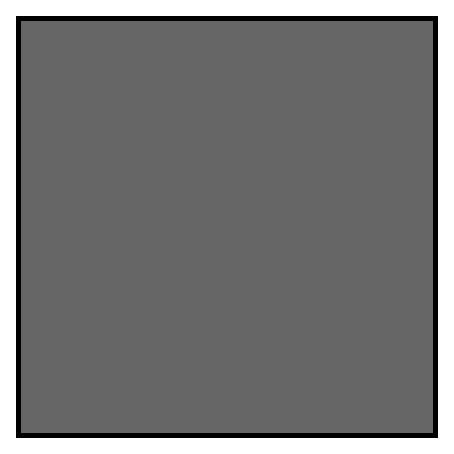
\includegraphics{example.eps}
% figure caption is below the figure
%\caption{Please write your figure caption here}
%\label{fig:1}       % Give a unique label
%\end{figure}
%
% For two-column wide figures use
%\begin{figure*}
% Use the relevant command to insert your figure file.
% For example, with the graphicx package use
%  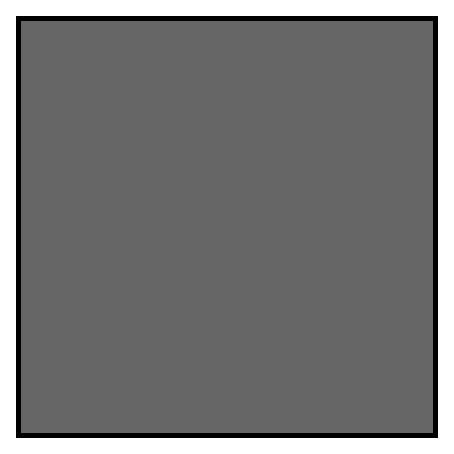
\includegraphics[width=0.75\textwidth]{example.eps}
% figure caption is below the figure
%\caption{Please write your figure caption here}
%\label{fig:2}       % Give a unique label
%\end{figure*}
%
% For tables use
%\begin{table}
% table caption is above the table
%\caption{Please write your table caption here}
%\label{tab:1}       % Give a unique label
% For LaTeX tables use
%\begin{tabular}{lll}
%\hline\noalign{\smallskip}
%first & second & third  \\
%\noalign{\smallskip}\hline\noalign{\smallskip}
%number & number & number \\
%number & number & number \\
%\noalign{\smallskip}\hline
%\end{tabular}
%\end{table}


%\begin{acknowledgements}

%\end{acknowledgements}

% BibTeX users please use one of
%\bibliographystyle{spbasic}      % basic style, author-year citations
%\bibliographystyle{spmpsci}      % mathematics and physical sciences
%\bibliographystyle{spphys}       % APS-like style for physics
\bibliographystyle{linquiry2} %use spbasic for journal of comparative gmc linguistics, etc.
\bibliography{joelrefs}   % name your BibTeX data base

\end{document}
% end of file template.tex

